%!TEX root = ../thesis.tex
\chapter{Реалізація моделі та аналіз результатів}
\label{chap:practice}

Щось про розділ


%%%%%%%%%%%%%%%%%%%%%%%%%%%%%%%%%%%%%%%%%%%%%%%%%%%%%%%%%%%%%%%%%%%%%%%%%%%%%%%%%%%


\section{Середовище}

Як основне середовище для розвитку організмів було створено 
просту реалізацію двовимірного обмеженого неперервного 
(в обчислювальному сенсі) середовища. 
Його ініціалізація проводиться низкою параметрів, 
таких як розміри середовища, розмір та енергетична цінність їжі, 
частота появи їжі, та інші. 
Середовище відповідає за низку процедур для моделювання: 
обробка результатів організмів, обробка колізій об’єктів, 
оновлення позицій об’єктів та моделювання плину часу в середовищі.


\begin{figure}[ht]
  \centering
  \caption{Візуалізація середовища}
  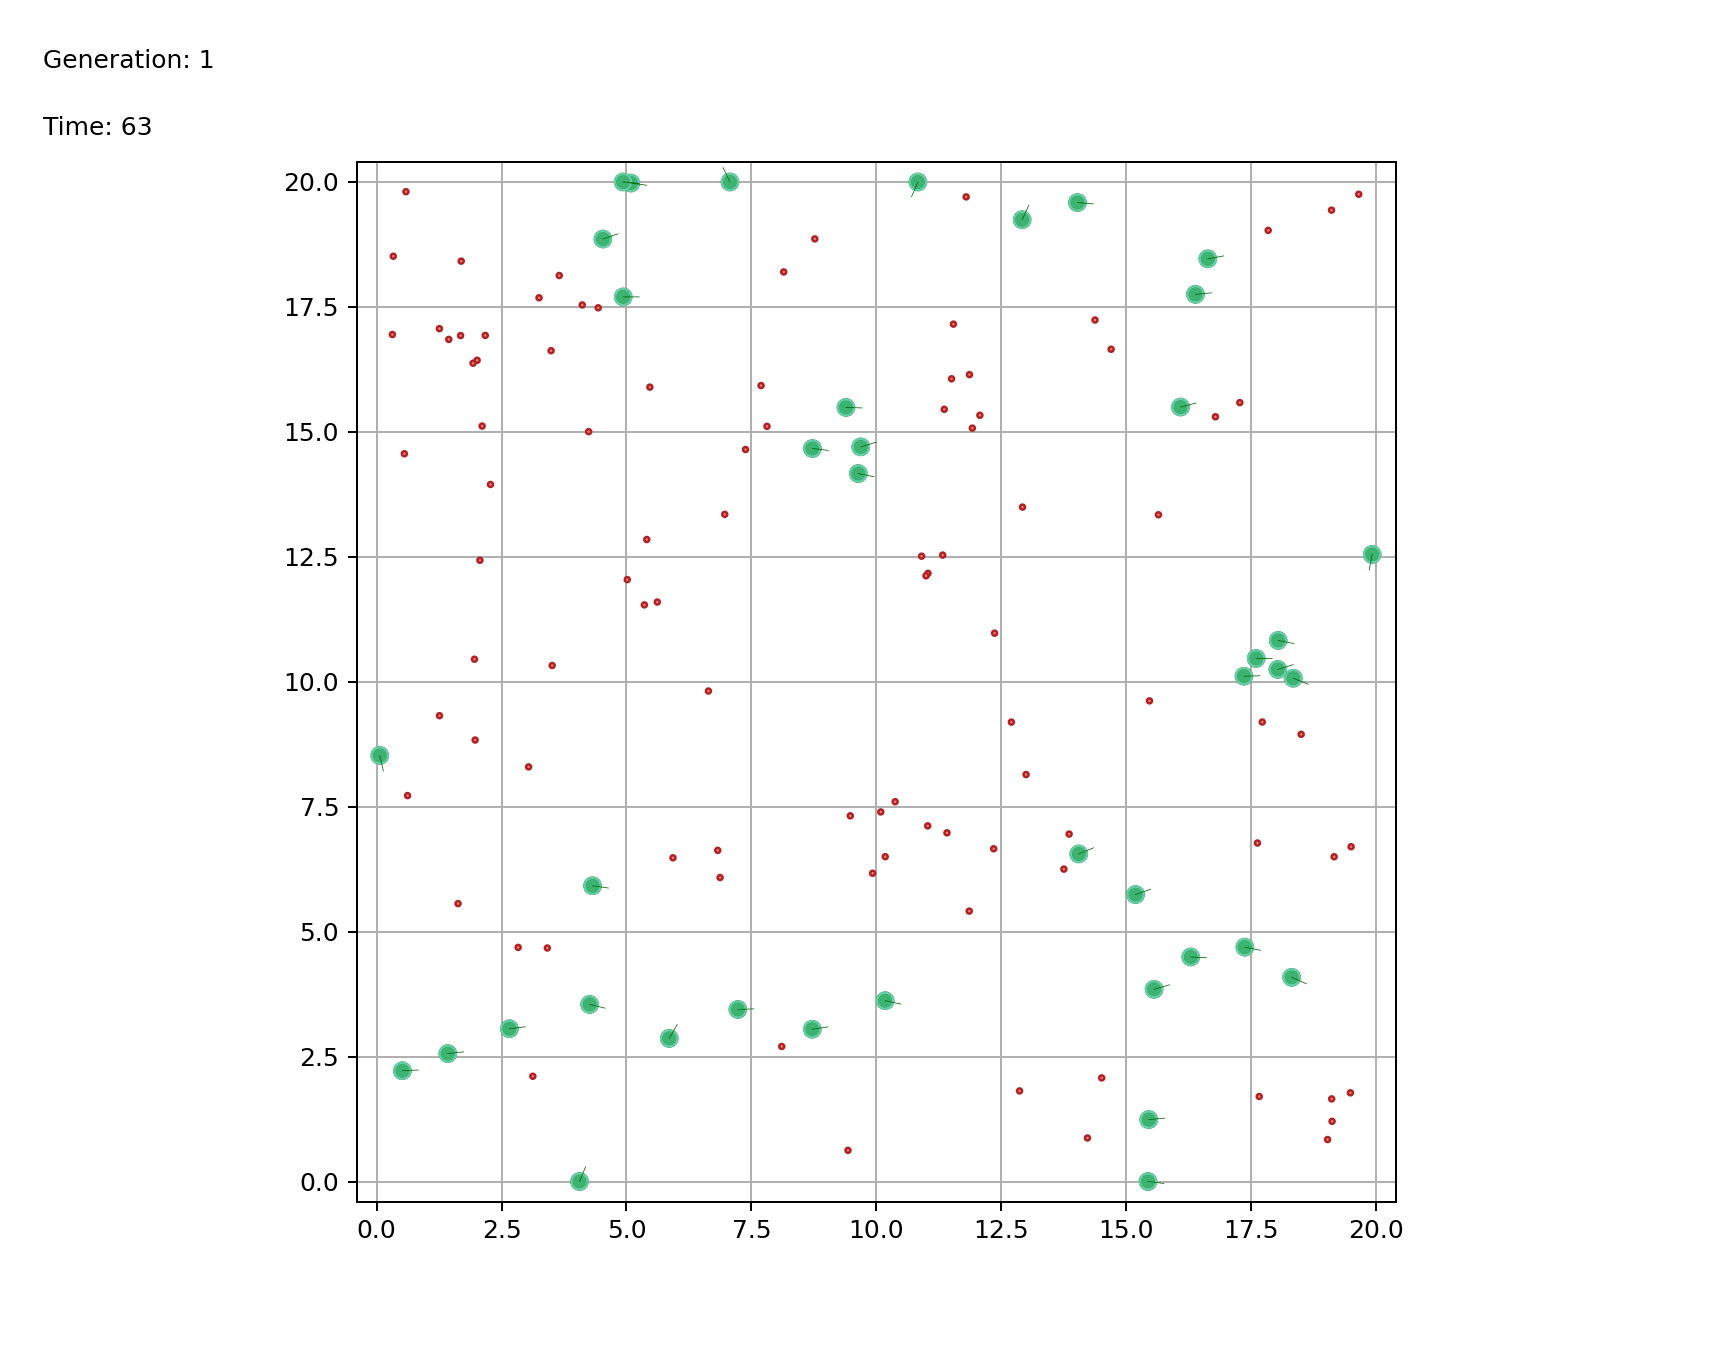
\includegraphics[scale=0.5]{Images/visualizing-the-environment.png}
  \label{fig:візуалізація-середовища}
\end{figure}


Для обробки колізій та ефективного зберігання об’єктів обрано 
просторову структуру даних R-Дерево (R-Tree). 
Ця структура зазвичай використовується для індексації 
багатовимірної інформації, такої як географічні координати, 
прямокутники або багатокутники.
Основною ідеєю цієї структури є ідея групування сусідніх 
об’єктів для представлення їх за допомогою мінімального 
обмежувального прямокутника на наступному вищому рівні дерева. 
Тому і має назву R-Tree, як дерево прямокутників.
Ця структура є корисною для практичних задач із просторовою взаємодією. 
В контексті Python існує бібліотека \verb+rtree+, 
що надає інтерфейс до вже реалізованої бібліотеки на C, 
що встановлюється на систему. 
Таким чином ми забезпечені достатньою швидкістю пошуку, 
зміни та інших маніпуляцій об’єктів у просторі.


Їжа грає ключову роль у процесі виживання та розвитку організмів, 
надаючи потрібний ресурс, що є розподіленим по середовищу. 
Сам об’єкт їжі є точкою з певним числом, 
що задає розмір цієї частинки. 
Кожна ця частинка має певну кількість енергії, 
що задається константно при ініціалізації середовища. 
Сама їжа у середовищі з’являється за ймовірнісним процесом. 
На старті середовища задається параметр для експоненційного розподілу, 
за яким і з’являються частинки у рівномірно вибраній точці середовища.
Також можливо обрати варіант появи їжі лише у певних
областях простору. Це зближує нас із реальною моделлю, оскільки 
природні ресурси, такі як їжа, часто розташовані у скупченнях 
через умови навколишнього середовища. 
Цього можна досягти за допомогою такого методу, як дискова вибірка Пуассона
\cite{bridsonFastPoissonDisk2007}.



%%%%%%%%%%%%%%%%%%%%%%%%%%%%%%%%%%%%%%%%%%%%%%%%%%%%%%%%%%%%%%%%%%%%%%%%%%%%%%%%%%
\section{Організми}

Об’єкт організму репрезентує модель біологічного індивіда, 
що має певний набір характеристик: геном, розмір, швидкість руху, 
прискорення, напрямок, енергетичний рівень, вік.

Геном організму задається парами матриць, 
що слугують вагами та упередженістю нейронної мережі. 
Сам клас самостійно оперує цією структурою. 
Єдина річ, яку потрібно задавати тут це шари нейронної 
мережі та кількість нейронів у них. 
Більша кількість шарів та нейронів призводить до більшого геному.

Кожен організм може думати за допомогою цієї мережі. 
Результат його праці --- це команда на пересування.
Кількість вихідних даних з мережі організму повинна
задаватися типом середовища моделювання.
Для тривимірного простору ми можемо задати шість ступенів свободи.
Все ж для поточної реалізації двовимірного простору
достатньо задати прискорення та зміну кута напряму.

Але кожна команда впирається у фізичні обмеження цього організму. 
Ми обмежуємо його пересування у середовищі задаючи максимальну 
можливу швидкість, прискорення та зміну напряму. 
Це є логічним, оскільки і в реальному житті будь-який 
організм не може змінити свої фізичні характеристики в одну мить. 
А в моделюванні з дискретним часом нам важливо зберегти якусь подібність до реальності.

На швидкості організм не повинен вміти швидко змінювати напрям. 
Саме тому додаємо гальмівний ефект від зміни напряму руху:
\[ v^{(t+1)} = \max(-v_{max}, \min(v_{max}, v^{(t)} + a)) \cdot \frac{1}{1 + d} \]


На обробку інформації про зовнішній світ у організма повинна 
якось змінюватися енергія. 
так ось і буде вона змінюватися за простим законом. 
вводимо коефіцієнт зміни енергії $\mu$ та будемо задавати зміну енергії так:
\[ E^{(t+1)} = E^{(t)} - \mu \cdot \left| \overline{o} \right| \]
Де $\overline{o}$ позначаємо як результат роботи нейронної мережі.

\hide{
Зовнішній світ повинен якось сприйматися організмом.
Наразі нейронні мережі сприймають зображення як матрицю
із закодованими значеннями кольорів.
Зображення по суті є проекцією тривимірних об'єктів.
Наші організми можуть розвиватися як у тривимірному просторі, так
і у двовимірному.
Ідеалістично, фенотип організму не повинен залежати від простору,
у якому він розвивається, але й зір є тісно пов'язаним із середовищем
та ідейно відноситься до об'єкта організму.
Тому кращим рішенням може бути відокремлення механізму зору від організма.
Це надає можливість тестувати довільну кількість таких імплементацій
навіть у одному процесі моделювання.
Такий механізм зору буде диктувати кількість нейронів у вхідному шарі мережі.

Візьмемо підхід, що буде перевикористовувати ідею цифрових зображень.
Зовнішній світ проектується на матрицю фіксованого розміру.
Надалі саме заповнення цієї матриці і залежить від конкретного
способу реалізації зору.
Зменшимо рівень абстракції "зору" до рівня кодування інформації навколо
об'єкта у матрицю фіксованого розміру.
Логічно використовувати набір позицій об'єктів у просторі
та їх фізичні властивості для створення матриці.
Кожен елемент у матриці буде кодувати відстань та напрямок
відносно <<голови>>  організму.
}

Організм повинен якось сприймати навколишнє середовище.
У реалізації Натана Руя \cite{rooyEvolvingSimpleOrganisms}
кожен організм на вхід приймав відстань та напрямок до найближчої
частинки їжу.
Ця модель не зовсім відповідає дійсності, оскільки
прорахунок найближчої цілі, напрям та відстань не отримується просто так.
Як і в житті, ми не бачимо точну відстань до предметів,
а приблизно оцінюємо ці відстань за допомогою орієнтування у просторі,
напруженні м'язів ока або відносній оцінці.
Тому потрібно надати найефективніше найближче сприйняття
до реальності.

Наразі нейронні мережі сприймають зображення як матрицю 
з закодованими значеннями кольорів.
По суті, зображення є проекцією об’єктів у трьох вимірах, тому й
наш механізм зору повинен надавати певну проекцію об'єктів на матрицю.
Ідеалістично, фенотип організму не повинен залежати від середовища, 
у якому він розвивається, але й зір має тісний зв’язок із 
середовищем та ідейно пов’язаний з об’єктом, у якому він знаходиться.
Також наші організми можуть розвиватися як у трьох, так і в двох вимірах.
Тому краще відокремити механізм зору від організму.
Це дозволяє тестувати будь-яку кількість таких імплементацій, 
навіть використовуючи один процес моделювання.
Кількість нейронів у вхідному шарі мережі буде визначена таким механізмом зору.

Виберемо стратегію, яка повторно використовує концепцію цифрових зображень.
Світ навколо організму проектується на матрицю певного розміру.
Заповнення цієї матриці також залежить від конкретного способу реалізації ідеї.
Зменшимо рівень абстракції «зору» до рівня кодування інформації навколо об’єкта в матрицю фіксованого розміру.
Логічно використовувати набір позицій об'єктів у просторі
та їх фізичні властивості для створення матриці.
Кожен елемент матриці закодує напрямок і відстань відносно «голови» організму,
а значення елемента можна подавати як тип об'єкта, де
для їжі ми ставимо одне константне значення, а для інших організмів
на шляху цільового --- інше.

\begin{figure}[ht]
    \centering
    \incfig{наповнення-матриці-для-механізму-зору}
    \caption{Наповнення матриці для механізму зору}
    \label{fig:наповнення-матриці-для-механізму-зору}
\end{figure}


%%%%%%%%%%%%%%%%%%%%%%%%%%%%%%%%%%%%%%%%%%%%%%%%%%%%%%%%%%%%%%%%%%%%%%%%%%%%%%%%
\section{Кодування}

Для генетичних алгоритмів використовують різні методи кодування, 
щоб представити розв'язки задачі в структурі хромосоми або геному. 
Типовими прикладами кодувань є: двійкове кодування, 
цілочисельне кодування, кодування дійсними числами, 
кодування перестановками та кодування значеннями.

Двійкове кодування представляє рішення за допомогою двійкових цифр (0 і 1). 
Якщо простір задачі вимагає дискретних величин, 
краще використовувати цілочисельне кодування, оскільки 
воно використовує цілі числа. Кодування перестановок підходить для 
проблем впорядкування або маршрутизації, 
оскільки воно передбачає розміщення речей або значень у певному порядку. 
У складних проблемних просторах, де певні стани або 
атрибути повинні бути представлені явно, кодування значень, 
також відоме як пряме кодування, передбачає безпосередній запис значень рішення.

У цій реалізації генетичного алгоритму для представлення геному організму 
можна конфігурувати різні можливі кодування. 
Це можливо завдяки правильній структурі коду, 
що дає можливіть швидко змінювати параметри моделі.

Але найкраще використати кодування дійсними числами. 
Перевага кодування в дійсних числах полягає в тому, 
що воно безпосередньо представляє неперервні змінні, що 
робить його особливо придатним для питань, 
пов'язаних з оптимізацією неперервного простору, 
таких як оптимізація ваг нейронних мереж.

Ваги та упередженність нейронної мережі безпосередньо кодуються в 
геномі організму за допомогою цього кодування в дійсних числах. 
Клас \verb+RealValued+ дає можливість кодувати та декодувати 
ваги організму в одновимірний масив геному. 
Для цього ваги та зсуви вирівнюються та об'єднуються. 
Для декодування сплющені масиви повертаються до початкових розмірів.

Завдяки такому кодуванню можна ефективно шукати у неперервному 
просторі оптимальні параметри нейронної мережі організму. 
Через те, що ваги та упередженність за своєю природою 
є дійсними числами, це забезпечує простий та ефективний 
метод оптимізації нейронних мереж. 
Імітуючи еволюцію біологічних організмів і використовуючи 
цей процес для вдосконалення моделей машинного навчання, 
ця методика втілює суть біологічно натхненного навчання.


%%%%%%%%%%%%%%%%%%%%%%%%%%%%%%%%%%%%%%%%%%%%%%%%%%%%%%%%%%%%%%%%%%%%%%%%%%%%%%%%%%
\section{Генетичні оператори}

Генетичні оператори грають величезну роль у зміні 
поведінки організмів та продуктивності генетичного алгоритму. 
Вони дозволяють вивчати можливі рішення проблеми у 
фазовому просторі рішень або ж перевикористати поточні 
варіанти для отримання більш кращого. 
Вибір і конфігурація цих операторів є важливою частиною 
проектування генетичного алгоритму.

Мутація вносить невеликі випадкові зміни в геноми індивідів, 
щоб підтримувати її різноманітність. 
Було запрограмовано різні типи мутації.

\verb+NonUniformMutation+ клас реалізує нерівномірну мутацію, 
яка змінює гени на основі функції, що зменшується з часом, 
сприяючи експлуатації, а не дослідженню в подальшому процесі роботи алгоритму. 
Це дозволяє на кінцевих ітераціях сфокосуватися на отриманні більш 
точних рішень, а ніж дослідженню простору.

\verb+GaussianMutation+ та \verb+UniformMutation+ є Гауссовую мутацією 
та рівномірною мутацією, які вносять зміни з нормального розподілу 
або з рівномірного розподілу відповідно.

Селекція --- це процес вибору особин, або батьків, 
які дадуть потомство у наступному поколінні. 
Клас \verb+TruncationSelection+ реалізує усічений відбір, 
який обирає найкращих $n$ особин на основі їхніх значень пристосованості. 
Цей підхід є простим і ефективним, гарантуючи, 
що для розмноження будуть обрані найбільш пристосовані особини.

Кросинговер --- ще один важливий генетичний оператор. 
Він дозволяє обмінюватися генетичним матеріалом між 
батьківськими особинами, створюючи таким чином потомство.

Клас \verb+SBXCrossover+ реалізує імітований двійковий 
кросинговер (SBX), який імітує поведінку одноточкового кросинговеру 
в генетичних алгоритмах з двійковим кодуванням в контексті кодування 
з дійсними значеннями. 
Він генерує нащадків ближче до батьків 
\cite{debSIMULATEDBINARYCROSSOVER, debSelfadaptiveSimulatedBinary2007}.

Клас \verb+BLXCrossover+ реалізує змішаний кросовер (BLX), 
який створює нащадків у діапазоні, визначеному генами батьків 
і пропорцією, що дозволяє проводити більш значні дослідження \hide{[5, 6].}
\cite{debSIMULATEDBINARYCROSSOVER}.

Клас \verb+ArithmeticCrossover+ генерує нащадків, 
використовуючи лінійну комбінацію генів батьків 
\cite{koraCrossoverOperatorsGenetic2017}.

Клас \verb+UniformCrossover+ реалізує простий рівномірний кросинговер,
де кожен ген нащадка випадковим чином вибирається від одного з батьків
\cite{koraCrossoverOperatorsGenetic2017}.


%%%%%%%%%%%%%%%%%%%%%%%%%%%%%%%%%%%%%%%%%%%%%%%%%%%%%%%%%%%%%%%%%%%%%%%%%%%%%%%%%%
\section{Опис інструментів та збір даних під час моделювання}

Механізм еволюції реалізовано з використанням 
об'єктно-орієнтованого підходу. 
По суті, це конвеєр, який перетворює популяцію організмів 
на наступне покоління. 
Цей процес відбувається в основному за допомогою чотирьох 
ключових кроків: відбору, проходження процесу елітизму, 
кросинговеру та мутації.

Також важливим параметром є ввімкнення процесу помирання 
організмів при досягненні критичної області енергії. 
Таким чином ми можемо отримати стаціонарний генетичний алгоритм, 
який не потребує переходів між популяціями,
змінюючи час на отримання наступної популяції та
кількість осіб у відборі. 
Його основна перевага це постійний процес еволюції, 
помирання індивідів та оптимізації по використанню пам’яті.

Було імплементовано комплексну бібліотеку для зручної роботи 
з дослідженням адаптації організмів до середовища. 
Підхід при її розробці мав на меті легку параметрицію для 
впровадження швидких експериментів по моделюванню життя організмів.

Також варто зазначити, що будь-яка частина програми може 
бути вільно замінена на іншу реалізацію. 
Тобто більш складні середовища можуть бути легко спровадженні у 
цей продукт через його модульність. 
Для дослідження цього проекту було вирішено обмежитися 
одним середовищем та одним типом організмів. 
Це дозволило швидко провести аналіз даних, отриманих за допомогою цієї моделі.

Сам же аналіз повинен здійснюватися по певних даних, які мають бути записані
під час процесу моделювання.
Такий запис повинен бути швидким по часу та займати мало постійної пам'яті,
тому на противагу запису в \verb+CSV+ файли було обрано \verb+Parquet+ тип.
Він має стовпчастий формат файлів для зберігання даних, націлений на обробку
великих масивів. Також забезпечуються ефективні алгоритми стиснення та кодування.

Для аналізу застосовувалися Jupyter Notebooks як середовище виконання коду.
У них відбувалося зчитування даних та візуалізація за допомогою 
бібліотеки для візуалізації даних \verb+plotly+.
Для більш адаптивного аналізу результатів багатьох запусків моделі із
різними параметрами використаний фреймворк \verb+dash+ 
для побудови веб-додатків для візуалізації даних.



%%%%%%%%%%%%%%%%%%%%%%%%%%%%%%%%%%%%%%%%%%%%%%%%%%%%%%%%%%%%%%%%%%%%%%%%%%%%%%
\section{Метрики}

Для аналізу поколінь організмів цілком розумно було б 
використати певний набів метрик, які б показали як 
поводять себе організми у середовищі, якою є їхня 
різноманітність та їх рівень розвитку. 
Використання цих метрик дасть можливість проводити більш 
обґрунтований та деталізований аналіз.

Однією з таких метрик є пристосованість, 
що у даній реалізації є не що інше як рівень енергії у організмі. 
Він надає інформацію про те, наскільки ефективно організм 
використовує доступні йому ресурси та його здатність 
адаптуватися до змін у навколишньому середовищі.

Також ми можемо задати метрику максимального та 
мінімального рівня енергії, що дасть нам більш повну 
інформацію про різноманітність популяції у використанні ресурсів.

Іншою є метрика співвідношення спожитої їжі до кількості 
рухів організму. 
Ця метрика допоможе нам зрозуміти енергоефективність організму, 
показуючи, наскільки ефективно він використовує отримані 
від їжі ресурси для своєї активності. 
Ця метрика обчислюється як відношення 
кількості рухів до кількості спожитих частинок їжі.

\todo[inline]{Metrics formulas}


%%%%%%%%%%%%%%%%%%%%%%%%%%%%%%%%%%%%%%%%%%%%%%%%%%%%%%%%%%%%%%%%%%%%%%%%%%%%%%%%%%
\section{Аналіз впливу параметрів по метрикам}

Дана модель може бути параметризована по:
\begin{enumerate}
  \item Розмірам середовища
  \item Тривалості одного покоління
  \item Типу зору організма
  \item Кількості енергії у частинках їжі та параметрам
    розподілу для генерації цим частинок
  \item Швидкості втрати організмами енергії при русі
  \item Методу відбору, мутації та рекомбінації
  \item Числу осіб, що переходять у наступну популяцію (елітизм)
  \item Розміру генома, що фактично означає кількості прихованих шарів
    та нейронів у них
  \item Кількості їжі, на старті
  \item Чи помиратимуть організми від нестачі енергії
  \item Параметрам нормального розподілу для генерації
    початкових ваг нейронної мережі
\end{enumerate}

%%%%%%%%%%%%%%%%%%%%%%%%%%%%%%%%%%%%%%%
% \todo[inline]{Які параметри розподілу для початкових геномів є кращими?}

Спочатку спробуємо відшукати кращі параметри для розподілу Гауса,
за допомогою якого генеруються початкові ваги нейронних мереж організмів.
Спочатку взято три варіанти для стандартного відхилення: 10, 1 та 0.1.
Математичне сподівання ж залишимо на рівні 0.

\begin{figure}[ht]
  \centering
  \caption{Отримані відношення спожитої їжі до руху при 
  пошуку кращого стандартного відхилення для генерації ваг}
  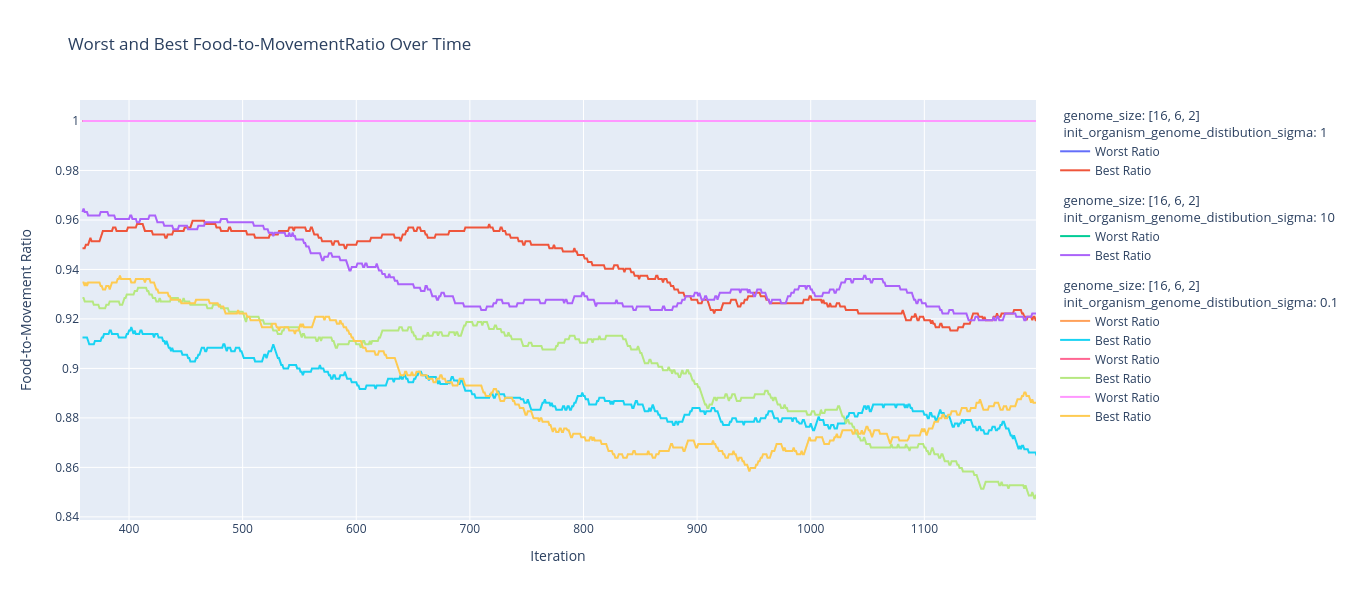
\includegraphics[scale=0.35]{Images/best_sigma_comparing_by_food_to_movement.png}
  \label{fig:отримані-відношення-спожитої-їжі-до-руху-при-пошуку-кращого-стандартного-відхилення-для-генерації-ваг}
\end{figure}

\begin{figure}[ht]
  \centering
  \caption{Рівні енергії при 
  пошуку кращого стандартного відхилення для генерації ваг}
  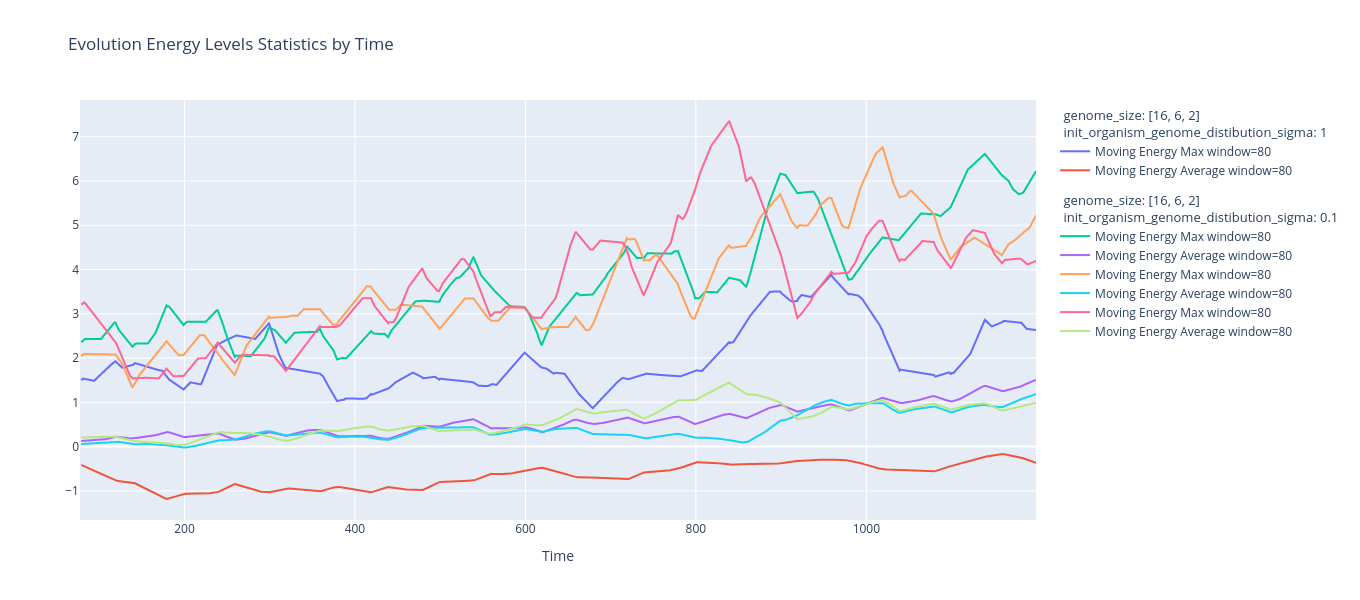
\includegraphics[scale=0.3]{Images/best_sigma_comparing_by_energy_levels.png}
  \label{fig:рівні-енергії-при-пошуку-кращого-стандартного-відхилення-для-генерації-ваг}
\end{figure}

З отриманого графіку \ref{fig:отримані-відношення-спожитої-їжі-до-руху-при-пошуку-кращого-стандартного-відхилення-для-генерації-ваг}
відношення спожитої їжі до руху бачимо помітну різницю
між організмами, що використовували 0.1 як стандартне відхилення, та іншими.
Також середній рівень енергії на графіку 
\ref{fig:рівні-енергії-при-пошуку-кращого-стандартного-відхилення-для-генерації-ваг}
у осіб з 0.1 стандартним відхиленням значно 
відрізняється від осіб з іншим параметром:
середня енергія значно вища, більша за нуль та зростає.
Отже область простору, де ми отримуємо значення геномів
зі стандартним відхиленням у 0.1 надає кращий старт для
життя організмів.



%%%%%%%%%%%%%%%%%%%%%%%%%%%%%%%%
% \todo[inline]{Які методи мутації та кросоверу дають кращий результат?}

Спробуємо підібрати гарну комбінацію методу рекомбінації
та мутації.
Оскільки у генетичних алгоритмах рекомбінація є центральним
елементом еволюції, то почнемо саме з неї.
Візьмемо декілька методів: BLX рекомбінація, Арифметична та
SBX із двома різними параметрами --- 1 та 2.
SBX рекомбінація при параметрі $n = 1$ буде мати
експлуатаційний характер, що дозволить мати пошук у локальній області.
Проаналізуємо графік середнього рівня енергії
по всім організмам впродовж часу.

\begin{figure}[ht]
  \centering
  \caption{Середній рівень енергії при 
  порівнянні методів рекомбінації}
  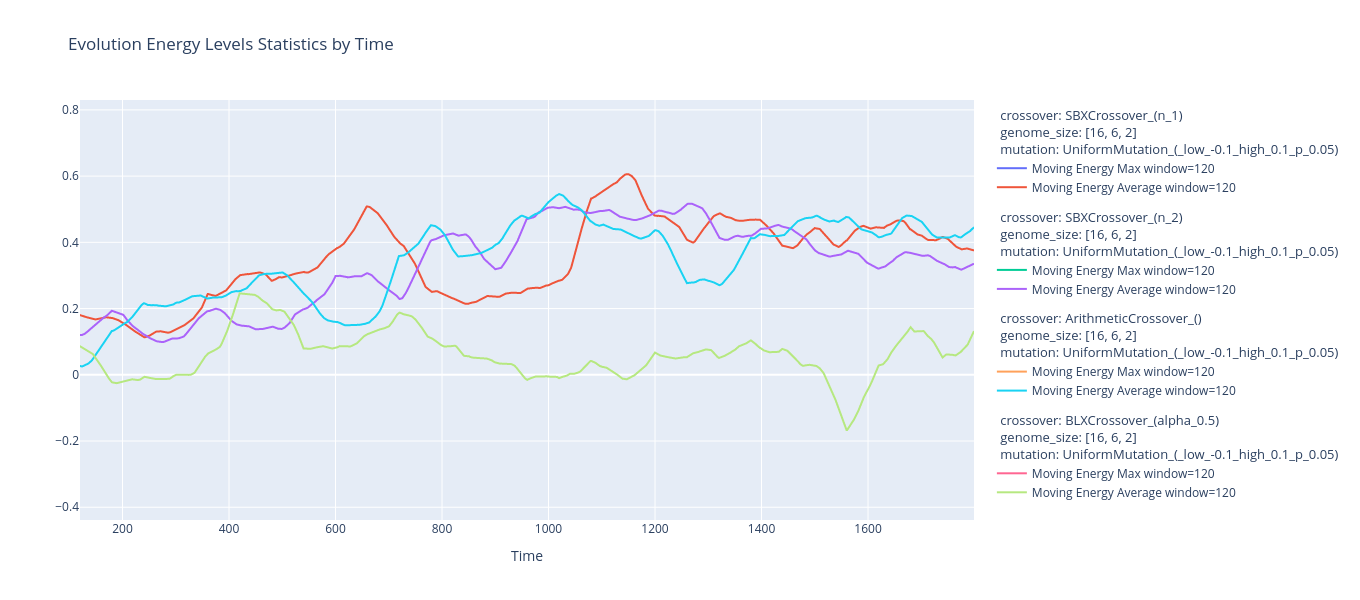
\includegraphics[scale=0.33]{Images/comparing_crossovers_sbx_arithmetic_blx05.png}
  \label{fig:середній-рівень-енергії-при-порівнянні-методів-рекомбінації}
\end{figure}

На графіку \ref{fig:середній-рівень-енергії-при-порівнянні-методів-рекомбінації}
більше всіх виділяється саме BLX рекомбінація із параметром $0.5$.
Він подає гірший результат у порівнянні з двома іншими.
А отже для наших цілей краще надалі використовувати
SBX або ж арифметичну рекомбінацію.

Вплив мутації не є настільки суттєвим та великим.
Під час попереднього моделювання не було помічено
випадку, коли певний метод мутації проявив себе краще, за інші.
Тому було обрано зупинитися на нерівномірній мутації через
її ідею на поліпшенні неявних рішень на завершальних ітераціях
алгоритму.



\todo[inline]{Яка кількість елітів та нащадків дають кращий результат?}



\todo[inline]{чи надає ускладнення форми організму йому переваги у життєдіяльності?}


Візьмемо такий набір кількості прихованих шарів з кількістю нейронів
нейронної мережі:
\begin{itemize}
  \item (6)
  \item (9)
  \item (9, 9)
  \item (18, 9)
\end{itemize}
З використанням 4 секцій дистанції та 4 секцій кута для зору
отримуємо 16 вхідних нейронів у кожній мережі. Також
на вихід маємо видавати два значення. Як результат маємо такий
набір нейронних мереж:
\begin{itemize}
  \item (16, 6, 2)
  \item (16, 9, 2)
  \item (16, 9, 9, 2)
  \item (16, 18, 9, 2)
\end{itemize}

При тестуванні роботи таких мереж отримали наступний графік рівнів енергії
та графік співвідношення спожитої їжі до руху:

\begin{figure}[ht]
  \centering
  \caption{Порівняння різних структур нейронних мереж організмів по максимальній енергії}
  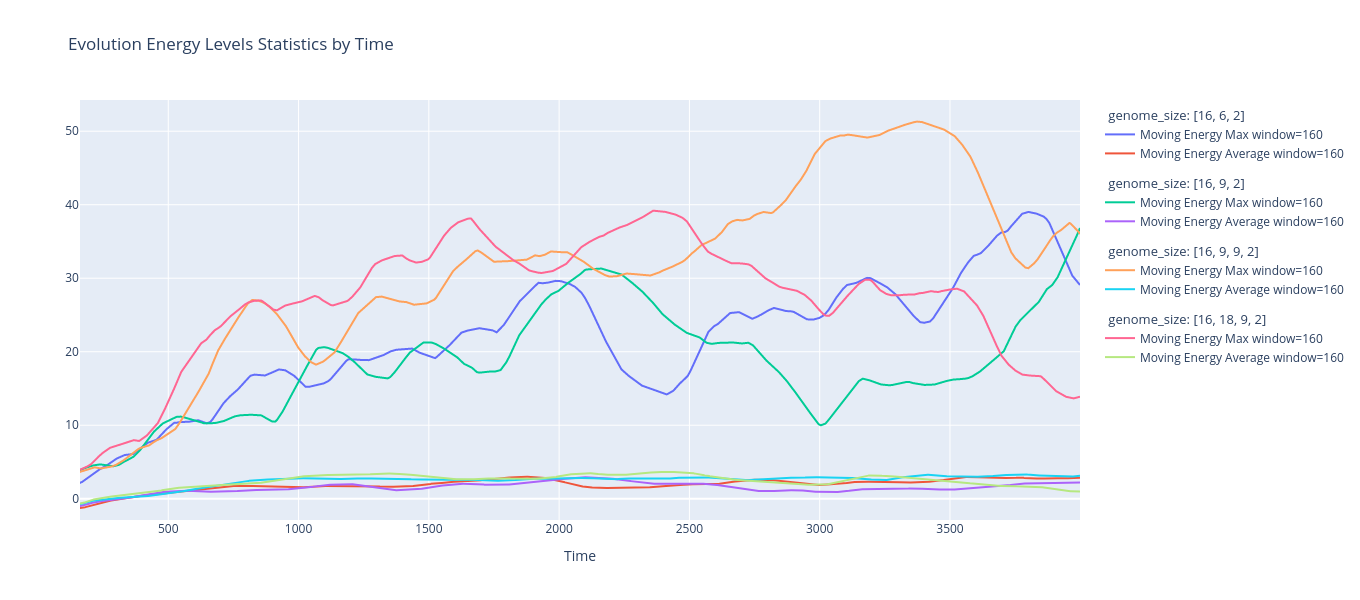
\includegraphics[scale=0.3]{Images/comparing-genomes-at-max-energy.png}
  \label{fig:порівняння-різних-структур-нейронних-мереж-організмів-по-амксимальній-енергії}
% \end{figure}

% \begin{figure}[ht]
  % \centering
  \caption{Порівняння різних структур нейронних мереж організмів по середньому значенню енергії}
  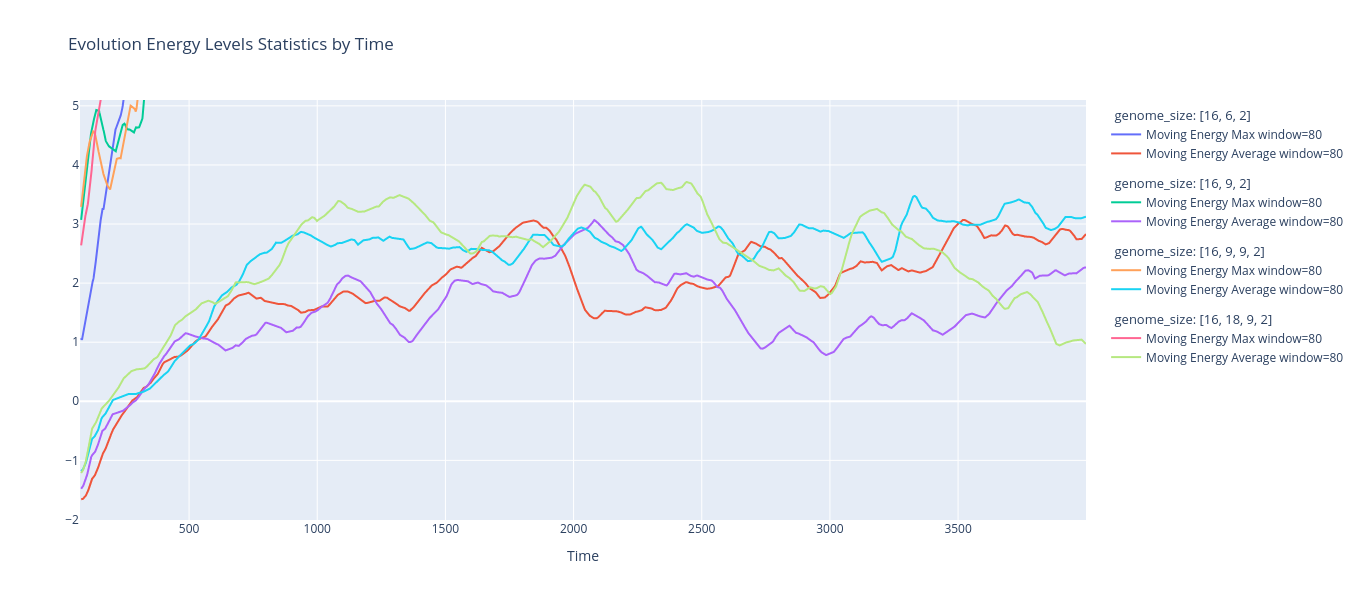
\includegraphics[scale=0.3]{Images/comparing-genomes-at-avg-energy.png}
  \label{fig:порівняння-різних-структур-нейронних-мереж-організмів-по-середньому-значенню-енергії}
\end{figure}

\begin{figure}[ht]
  \centering
  \caption{Порівняння різних структур нейронних мереж організмів по відношенню спожитої їжі до руху}
  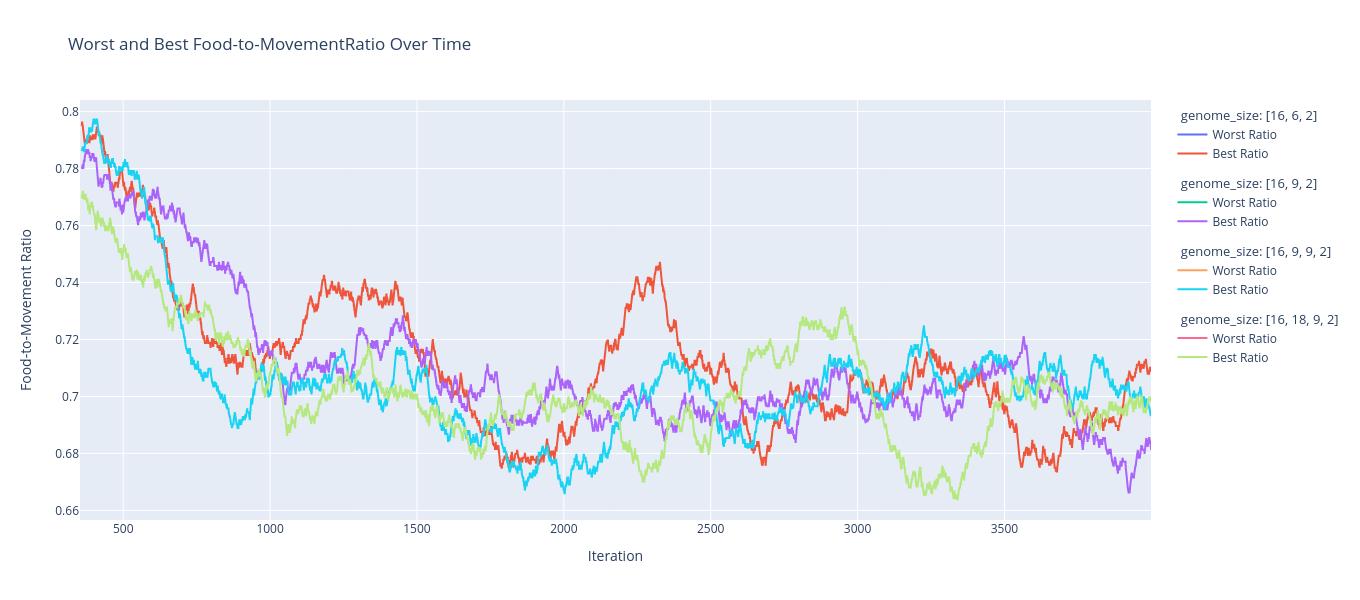
\includegraphics[scale=0.3]{Images/comparing-genomes-at-food-to-movement.png}
  \label{fig:порівняння-різних-структур-нейронних-мереж-організмів-по-відношенню-спожитої-їжі-до-руху}
\end{figure}

З графіку
\ref{fig:порівняння-різних-структур-нейронних-мереж-організмів-по-відношенню-спожитої-їжі-до-руху} 
суттєвої різниці між діями організмів не видно.
А отже навчаються вони досить однаково.

По значенню максимальної кількості енергії
\ref{fig:порівняння-різних-структур-нейронних-мереж-організмів-по-амксимальній-енергії}
схоже, що у індивідів популяції
з більш складнішиою структурою існують індивіди,
що здатні спожити більшу кількість їжі.
Це може означати, що вони розвинули більш досконалі або
ефективні методи використання енергії їжі.
Така поведінка пояснюється збільшенням кількості нейронів,
що могло призвести до покращення здатності вирішувати проблеми
та більш ефективної адаптації до навколишнього середовища.

Однозначно стверджувати, який варіант організмів ми поки не можемо.
Кількість нейронів для простих організмів може бути не на достатньому рівні,
щоб швидко отримати потрібні знання для утилізації частинок їжі.
Спробуємо порівняти із більш складним організмом на рівні
(16, 18, 9, 9, 2) шарів нейронної мережі.


\begin{figure}[ht]
  \centering
  \caption{Порівняння простої та складної структури нейронної мережі організмів по енергії}
  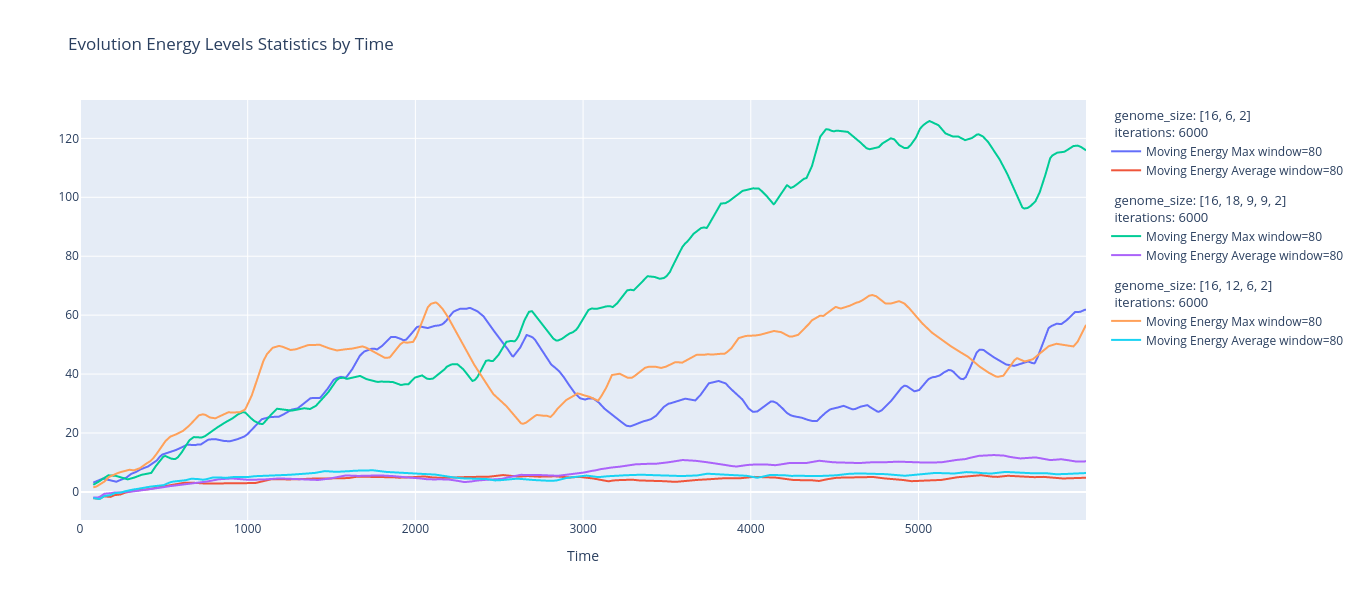
\includegraphics[scale=0.3]{Images/comparing-genomes-energy-levels-complex-is-leader.png}
  \label{fig:порівняння-простої-та-складної-структури-нейронної-мережі-організмів-по-енергії}
\end{figure}

По графіку \ref{fig:порівняння-простої-та-складної-структури-нейронної-мережі-організмів-по-енергії}
можемо проаналізувати, що простіші структури виявилися кращими на початкових
етапах розвитку організмів.
Вони змогли вдосталь пристосуватися для отримання певної кількості енергії
у короткостроковій перспективі.
Але надалі їх розвиток сповільнився.
У той же час складна структура (16, 18, 9, 9, 2) отримувала дані
про навколишній простір та зробила сильний ривок
за рівнем максимальної кількості енергії,
випереджаючи свої простіші аналоги.
По рівню середньої енергії по популяції ця структура має також вищі показники.


На перший погляд, простіші структури отримують більше їжі 
пропорційно до кількості руху та тримають достатній рівень
енергії для виживання на певний період. 
Однак з часом результати роботи як простих, 
так і складних систем змінюються, що 
свідчить про важливість навчання та адаптації в обох типах структур.

\begin{figure}[ht]
  \centering
  \caption{Порівняння простої та складної структури нейронної мережі організмів по відношенню спожитої їжі до руху}
  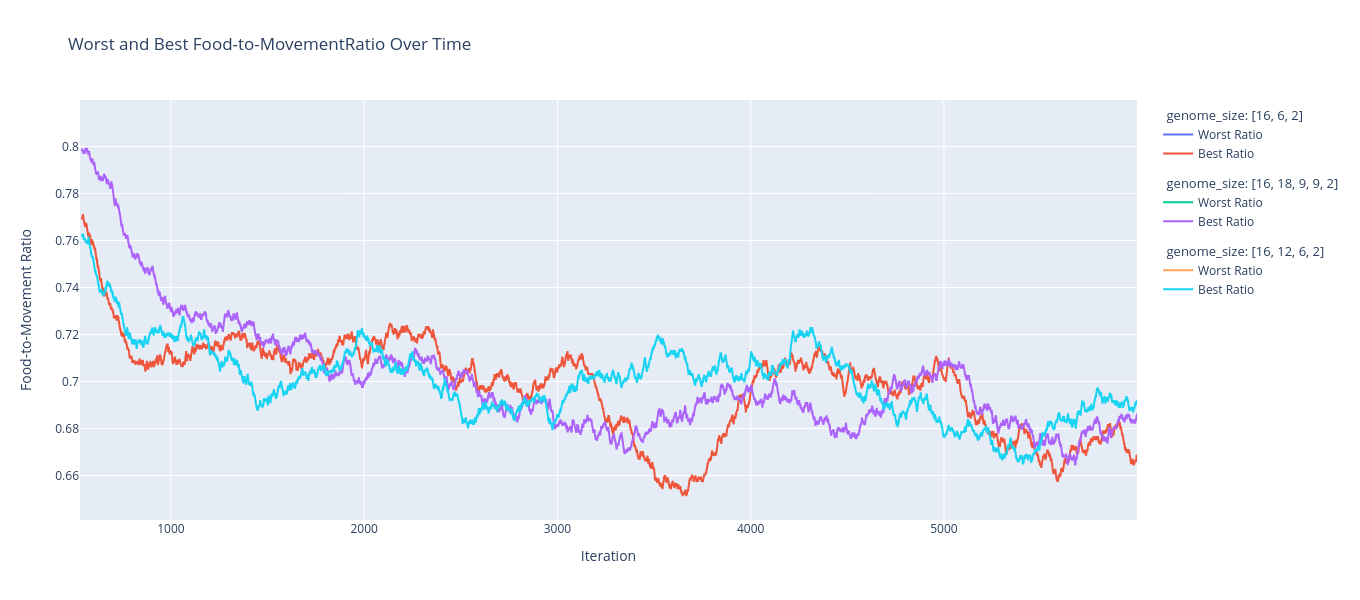
\includegraphics[scale=0.3]{Images/comparing-genomes-food-to-movement-complex-is-leader.png}
  \label{fig:порівняння-простої-та-складної-структури-нейронної-мережі-організмів-по-відношенню-спожитої-їжі-до-руху}
\end{figure}

По графіку відношення спожитої їжі до руху
\ref{fig:порівняння-простої-та-складної-структури-нейронної-мережі-організмів-по-відношенню-спожитої-їжі-до-руху}
чітко видно, як на початкових стадіях розвитку організмів
простіша структура отримує більше їжі, по відношенню до кількості рухів,
але надалі обидва варіанти структур показують перемінний результат.

Такі результати можна пояснити через структурну складність 
конфігурації з більшою кількістю шарів нейронної мережі. 
Через збільшення шарів у мережі організм містить довший геном, 
а отже збіжність популяції з такою структурою може бути повільнішою, 
порівнюючи її з популяцією з меншим геномом.
Оскільки існує менше змінних і менший простір для 
пошуку оптимальних генетичних комбінацій, 
коротші геноми з простішою архітектурою можуть забезпечити 
швидшу адаптацію. 
Як наслідок, менші структури можуть знайти ефективний 
спосіб споживання енергії швидше, ніж їхні складніші аналоги.

Коротший геном дозволив популяції знайти оптимальні рішення 
до отримання все більших запасів енергії за короткий проміжок часу. 
Але популяція з довшим геномом також навчається та 
може вмістити у геном більше інформації для реагування 
на різні події у їхньому житті,
оскільки довший геном забезпечує більшу
різноманітність генетичних комбінацій і, 
як наслідок, більшу можливість для довготривалої адаптації. 
Організмам зі складною структурою може знадобитися більше часу для 
визначення оптимального набору генетичних конфігурацій,
оскільки їх область пошуку є значно більшою. 
Але після цього вони мають потенціал для адаптації до ширшого діапазону 
умов та оптимізації споживання енергії в більшій мірі, ніж простіші структури.
При зміні правил середовища ці знання можуть зіграти свою роль.



%%%%%%%%%%%%%%%%%%%%%%%%%%%%%%%%%%%%%%
% \todo[inline]{ чи спостерігаються паттерни групової свідомості (ройового штучного інтелекту) в поведінці групи?  }


Організми можуть скупчуватися у групи за певних умов.
З мисленого експерменту можна стверджувати, що подібне
скупчення у групи може відбуватися лише при виконанні
як мінімум однієї з двох умов:
\begin{enumerate}
  \item механізм зору в організмів дозволяє їм бачити
    собі подібних;
  \item під час еволюції організми можеть досягти стадії розвитку,
    коли їх поведінка на зовнішні подразники (частинки їжі або інші організми)
    буде мати схожий характер у межах групи.
\end{enumerate}

Хоча й методи розпізнавання та схожа поведінка можуть відігравати важливу роль,
та у формуванні групи можуть діяти й інші процеси.
Наприклад, процес комунікації, спільні способи захисту або добування їжі ---
все може сприяти формуванню групи.
Але такі процеси відносяться до більш складних моделей та реальній моделі
розвитку організмів.

\begin{figure}[ht]
  \centering
  \caption{Утворення групи організмів}
  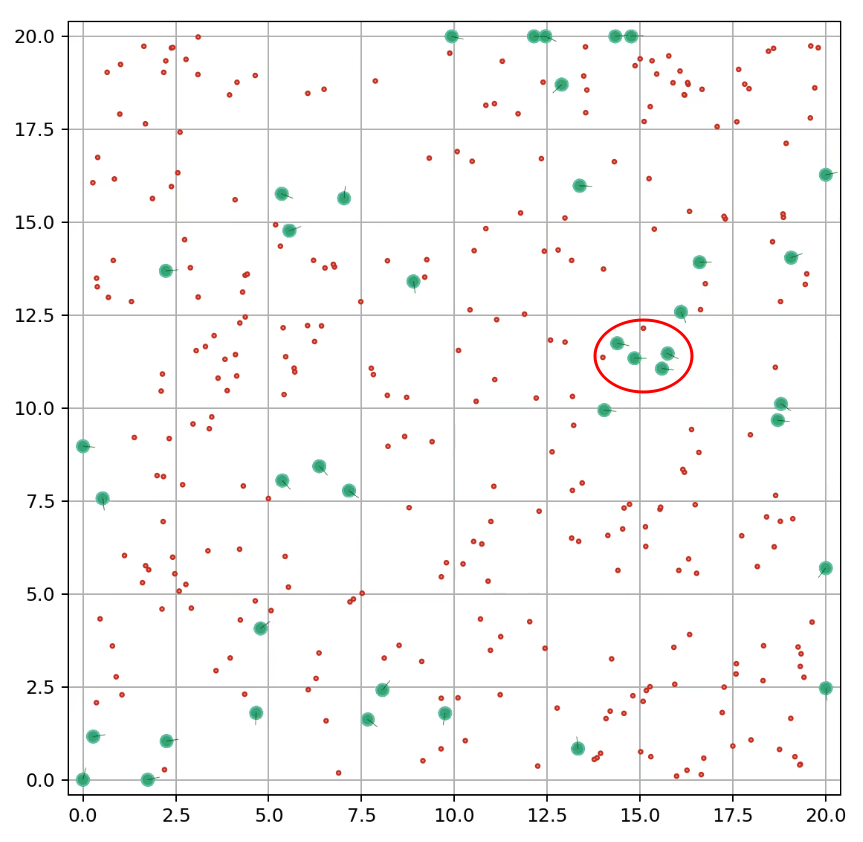
\includegraphics[scale=0.5]{Images/organisms-group-of-4.png}
  \label{fig:утворення-групи-організмів}
\end{figure}

Звичайно, таку складну ідеалізовану модель важко реалізувати,
що беззаперечно дає визнання складності реальних умов.
Та все ж під час спостереження за розвитком організмів під час експерименту
було помічено малі групи індивідів, що рухали за схожим шаблоном.
Часто саме присутність аналогічного організму поряд
давала поштовх змінити курс та слідувати за ним.
Це надає переконливі емпіричні докази групової поведінки,
навіть якщо ці угрупування не дають переваги у такому конкурентному
середовищі.
Часто саме такі групи помирали, оскільки пошук їжі у такому бідному середовищі
вимагає змагання із усіма, навіть із учасниками групи.






%%%%%%%%%%%%%%%%%%%%%%%%%%%%%%%%%%%%%%%%%%%%%%%%%%%%%%%%%%%%%%%%%%%%%%%%%%%%%%%%%%
% \hide{

% Зазвичай третій розділ присвячено опису практичного застосування або 
% експериментальної перевірки аналітичних результатів, одержаних у другому 
% розділі роботи. Втім, це не обов'язкова вимога, і структура основної 
% частини диплому більш суттєво залежить від характеру поставлених завдань. 
% Навіть якщо у вас є певне експериментальне дослідження, але його загальний 
% опис займає дві сторінки, то краще приєднайте його підроздіром у 
% попередній розділ.

% При описі експериментальних досліджень необхідно:

% \begin{itemize}
% \item наводити повний опис експериментів, які проводились, параметрів 
% обчислювальних середовищ, засобів програмування тощо;
% \item наводити повний перелік одержаних результатів у чисельному вигляді для їх можливої 
% перевірки іншими особами;
% \item представляти одержані результати у вигляді таблиць та графіків, 
% зрозумілих людському оку;
% \item інтерпретувати одержані результати з точки зору поставленої задачі 
% та загальної проблематики ваших досліджень.
% \end{itemize}

% У жодному разі не потрібно вставляти у даний розділ тексти 
% інструментальних програм та засобів (окрім того рідкісного випадку, коли 
% саме тексти програм і є результатом проведення експериментів). За 
% необхідності тексти програм наводяться у додатках.

% }
%%%%%%%%%%%%%%%%%%%%%%%%%%%%%%%%%%%%%%%%%%%%%%%%%%%%%%%%%%%%%%%%%%%%%%%%%%%%%%%%%%%

\chapconclude{\ref{chap:practice}}


% Ця робота забезпечила поглиблене вивчення моделі на 
% основі генетичного алгоритму,
% яка імітує еволюцію організмів у віртуальному середовищі. 

Модель репрезентує просту абстракцію реального механізму розвитку організмів,
але не є повним еквівалентом, хоча і поділяє кілька основних концепцій.
Дана модель наслідує механізми виживання та кількості енергії:
реальні біологічні організми споживають певні ресурси, що надають їм можливість
виживати. Цей принцип є фундаментальним у такій моделі.
Подібно до справжньої біологічної еволюції, 
модель використовує генетичні алгоритми для імітації концепцій 
природного відбору, мутацій та успадкування. 
Нейронна мережа є абстрактною картиною того,
як реальні істоти використовують свій генетичний код
для створення складних дій та функцій.
Те, як нейронна мережа використовується
для відтворення процесу <<мислення>> організму,
схоже на те, як реальні тварини використовують
свій мозок для взаємодії з навколишнім середовищем.
Однак важливо зазначити, що спрощення та абстракції, 
необхідні для комп'ютерного моделювання означають, 
що дана модель не є ідеальним відображенням реального світу
через обмеження у: сенсорах, спрощеному середовищі,
відсутності росту, складності геному.


Дослідження виявило динамічний зв'язок між складністю геному, 
швидкістю еволюції та довгостроковою адаптацією. 
Підібрані гарні параметри для старту моделювання та механізми
еволюції.
Було показано, що організми з простішою генетичною архітектурою адаптуються 
швидше через менший простір рішень. 
Однак, незважаючи на більш повільну початкову еволюцію, 
індивіди зі складнішою архітектурою геному демонстрували кращий потенціал 
для довгострокової адаптації.
Цікаво, що, незважаючи на простоту моделі, було виявлено
зачатки розвитку груп у популяції. 

% Дослідження також висвітлило труднощі, пов'язані з дефіцитом 
% ресурсів, оскільки групи часто гинули через труднощі в отриманні їжі, 
% що підкреслює компроміс між соціальною поведінкою 
% та конкурентною боротьбою за ресурси. 
% Це узгоджується з тенденціями, що спостерігаються в біологічних системах, 
% і підкреслює необхідність додаткових досліджень еволюції кооперативних 
% або взаємовигідних дій у відповідь на екологічні обмеження.

% Результати дослідження демонструють потужність генетичних алгоритмів 
% у відтворенні складних біологічних процесів, 
% які є результатом простих еволюційних механізмів. 
% Проект підкреслює корисність еволюційних обчислень як інструменту 
% для розуміння біологічної еволюції та 
% вдосконалення складних систем штучного інтелекту.

% Загалом, це дослідження закладає основу для майбутніх 
% досліджень еволюційної динаміки, зокрема, 
% впливу змін умов навколишнього середовища та генетичної складності 
% на адаптацію та стратегії виживання організмів.


% \todo[inline]{
% - чи відображає модель з достатньою точністю поведінку реальних систем? (так, навести приклади, якщо зможете)

% - чи надає ускладнення форми організму йому переваги у життєдіяльності? (парадоксально, але не завжди - прості, але швидкі і прожерливі організми швидше накопичують вагу)

% - чи спостерігаються паттерни групової свідомості (ройового штучного інтелекту) в поведінці групи? (про певні залежності можна говорити, але потрібні додаткові обчислювальні експерименти. якщо щось спостерігалося - можна вказати)
% }
